\documentclass[11pt]{article} % For LaTeX2e
\usepackage{rldmsubmit,palatino}
\usepackage{graphicx}
\usepackage{caption}
\usepackage{subcaption}
\usepackage[round]{natbib}


\title{The formation of habits: a computational model mixing reinforcement and Hebbian learning}


\author{
Meropi Topalidou \\
INRIA Bordeaux Sud-Ouest, Bordeaux, France\\
Universit{\'e} de Bordeaux, CNRS UMR 5293, IMN, France \\
LaBRI, Universit{\'e} de Bordeaux, IPB, CNRS, UMR 5800, Talence, France\\
\texttt{meropi.topalidou@inria.fr} \\
\And
Daisuke Kase\\
Universit{\'e} de Bordeaux, CNRS UMR 5293, IMN, France \\
Laboratoire Franco-Isra{\'e}lien de Neurosciences, CNRS Bordeaux, France \\
\texttt{daisuke.kase@u-bordeaux.fr} \\
\AND
Thomas Boraud \\
Universit{\'e} de Bordeaux, CNRS UMR 5293, IMN, France \\
\texttt{thomas.boraud@u-bordeaux.fr} \\
\And
Nicolas Rougier \\
INRIA Bordeaux Sud-Ouest, Bordeaux, France\\
Universit{\'e} de Bordeaux, CNRS UMR 5293, IMN, France \\
LaBRI, Universit{\'e} de Bordeaux, IPB, CNRS, UMR 5800, Talence, France\\
\texttt{nicolas.rougier@inria.fr}
}

% The \author macro works with any number of authors. There are two commands
% used to separate the names and addresses of multiple authors: \And and \AND.
%
% Using \And between authors leaves it to \LaTeX{} to determine where to break
% the lines. Using \AND forces a linebreak at that point. So, if \LaTeX{}
% puts 3 of 4 authors names on the first line, and the last on the second
% line, try using \AND instead of \And before the third author name.

\newcommand{\fix}{\marginpar{FIX}}
\newcommand{\new}{\marginpar{NEW}}

\begin{document}

\maketitle

\begin{abstract}
If basal ganglia are widely accepted to participate in the high-level cognitive function of decision-making, their role is less clear regarding the formation of habits. One of the biggest problem is to understand how goal-directed actions are transformed into habitual responses, or, said differently, how an animal can shift from an action-outcome (A-O) system to a stimulus-response (S-R) one while keeping a consistent behavior.

We introduce a computational model (basal ganglia, thalamus and cortex) that can solve a simple two arm-bandit task using reinforcement learning and explicit valuation of the outcome (Guthrie et al., 2013). Hebbian learning has been added at the cortical level such that the model learns each time a move is issued, rewarded or not. Then, by inhibiting the output nuclei of the model (GPi), we show how learning has been transfered from the basal ganglia to the cortex, simply as a consequence of the statistics of the choice. Because best (in the sense of most rewarded) actions are chosen more often, this directly impacts the amount of Hebbian learning and lead to the formation of habits within the cortex.

These results have been confirmed in monkeys (unpublished data at the time of writing) doing the same tasks where the BG has been inactivated using muscimol. This tends to show that the basal ganglia implicitely teach the cortex in order for it to learn the values of new options. In the end, the cortex is able to solve the task perfectly, even if it exhibits slower reaction times.
\end{abstract}

\keywords{basal ganglia, decision making, habits, reward, Hebbian learning, reinforcement learning}

% \acknowledgements{}

\startmain % to start the main 1-4 pages of the submission.

\section{Introduction}

	A lot of times during a day, we are asked to make decisions of different kind, important or not. Each of these decisions show who we are, through influencing our behaviour and habits. Nowadays, many scientists are involved in research of understanding the underlying mechanisms of this high-level cognitive function. It is a widely held view that basal ganglia participate in decision making, but with unknown role regarding the formations of habits. How an animal can shift from a known behaviour with expected outcome to a habitual one?
	
	Piron experimented with monkeys on a two-armed bandit task under a pharmacological approach, combining habitual behaviour and procedural learning. In this kind of tasks, the subjects are requested to determine the initial unknown outcome of a choice among different options. During a trial, two different shapes are presented to a screen in front of a monkey. Each shape is interlaced with a reward probability (0.75 and 0.25). Its task is to choose one by pushing a button relevant to the position of the shape. Finish of the movement indicates reward delivery according to chosen shape's probability. Through repetition, the monkey decodes the hidden outcomes and chooses almost each time the shape with the highest one. Then, they interchange between trials with familiar targets of explicit values and new pairs of targets of implicit value. A reflexive behaviour was triggered by the former trials in which the choice was the best option and quick, while the later are associated to an exploratory early phase and a late exploitation phase of a learning process. Yet, they inactivated the internal part of the Globus Pallidus (GPi), the main output structure of the BG with injections of muscimol. They concluded that disruption of BG output resulted to inability of learning new contingencies, while the reflexive choice of known target was slightly slower, but not impaired.

	We introduce a computation model that simulates cortex, basal ganglia and thalamus, able to solve the two-armed bandit task, as described above, using reinforcement learning and explicit valuation of outcome (Guthrie et al., 2013). Our results demonstrate that Hebbian learning at cortical level after each move, and not only after reward, is sufficient for the model to choose always the best option. Then, by inhibiting the output nuclei of the model (GPi), we show how learning has been transferred from the basal ganglia to the cortex, simply as a consequence of the statistics of the choice. Our results are consisted with equivalent monkeys' experiments (unpublished data at the time of writing) and suggest that the basal ganglia implicitly teach cortex the values of new options. In the end, it is demonstrated the ability of cortex to solve the task perfectly, even if it exhibits slower reaction times.
\section{Description of the model}

The architectural basis of the model has been originally described in
\citet{Guthrie2013} where authors introduced a biophysical model of action
selection that can solve a two-armed bandit task. Two parallel action selection
patways compose the model with inputs from distinct areas of the cortex: one
for dealing with the cognitive action selection, and the other for the motor
one. The model includes the cortex (Cx), Thalamus (Th) and several nuclei of
the BG: Striatum (Str), Subthalamus (STN), Globus pallidus (GPi). Each module
is made of a closed-loop positive feedback direct pathway (Cx-Str-GPi-Th-Cx)
and a closed-loop negative feedback hyperdirect pathway (Cx-STN-GPi-Th-Cx) and
is based on the a the center-surround architecture of \cite{Mink:1996}. The
interaction between these two pathways is able to induce an action selection at
the motor level. However, the task requires first the actual selection of the
best cue before performing the corresponding motor action. In the
\citet{Guthrie2013} model, this is implemented at the striatal level where a
dopamine reward signal is used to implement a simple value-based learning. The
general architectural of the model is illustrated on figure \ref{fig:architecture}.

However, in the original model, the inactivation of basal ganglia output (GPi)
results in the inability of the model to make a decision because there is no
competiting mechanism at the cortical level. We thus added lateral connections
in each cortical modules (self-excitation and surround inhbition) such that a
unique cognitive and motor decision can be made. However, at this stage, there
is no guarantee that the motor decision corresponds to the cognitive ones. The
model can choose cue A but moves toward location of cue B. To overcome this
problem, we also need to establish a cross-talking between the different
cortical modules, independently of BG pathways. This has been made using
excitatory connections from and to the associative cortical module. With proper
learning, this allow the cortex to make a consistent decision in the absence of
GPi, even if it does not guarantee to make the optimal decision.

One important property of the cortical decision is that it is significantly
slower than the BG decision. This can be shown by measuring the time of motor
decision, which has been defined at the time where the difference between the
two most activated units in the motor cortex is greater than a given threshold
(40Hz). Before learning, the BG decision time (GPi is intact) is around 250ms
while the cortical decision time (GPi is disabled) is around 800 ms. This
difference in timing is actually critical for the BG to teach the cortex as
explained in the results section.


%% module. Consequently, inactivation of the GPi automatically means the loss of this
%% ability.  Yet, Guthrie model did not provide time to cognitive cortex for
%% making a decision, before motor decides the appropriate move. They are a lot of
%% cases that the two decisions are simultaneously, even the motor before the
%% cognitive, at some cases. In order to obtain this difference in timing, except
%% the added connections, a part of the original parameters have changed.


%% One of the results from experiments by \citet{Piron2015}, was the success of
%% monkeys to reserve their knowledge after inactivation of GPi. This is a strong
%% indication for storage of information outside of basal ganglia. It's known that
%% striatal learning follows the rules of reinforcement learning. Each time BG
%% computes the expected reward of an action and adjusts the weights according to
%% the error of the real one. In the opposite side is the cortical learning about
%% which our knowledge is limited. We hypothesized that learning occurs after
%% every move without the need of any computation or outcome. Therefore, hebbian
%% learning is a good candidate. The success of this choice is ensured by the
%% participation of BG to the action selection. After few trials, BG learn the
%% best option and guide cortex to choose it. In this way, the number of choice of
%% the cues are capable, through the statistics, to drive cortex to learn
%% properly. This is also confirmed by the absence of GPi, when cortex is
%% incapable to learn new strategies. At that point, choices are statistically
%% random, so the learning is balanced between the two cues.

\section{Results}

	The main task at the experiments by Piron was a two-armed bandit paradigm. During an exploratory phase by trial and errors, the monkeys appraise what are the outcomes (various probability of reward in most of the cases). Afterwards, they choose preferentially the best option (maximizes the reward). Most of the species don't have this ability to conclude the outcome, and for those that do have it (primates amongst them), it takes more than one session of training. 
	First, only two cues were always presented to the monkey, with probabilities of reward 0.75 and 0.25. After the learning phase, a testing one followed. Now, a pair of cues of which they know the values or  a new set of cues of unknown values was presented. By pharmacological approach, they tested with and without inactivation of the major output of basal ganglia, Globus Pallidus (GPi), toward the cortex through the thalamus in order to unravel their role in decision making and learning processes.
	For testing our model, we followed the protocol by Piron. There were 50 trials in the learning phase in order the network to learn the two according to their reward probabilities. Followed by the testing, which comprising of 20 trials presenting a set of cues with known values and 20 with a pair of unknown, with or without active GPi.
	Our results were in accordance with the ones of the experiments. Figure \ref{fig:Performances} shows that the network maximizes its choice at known values cues in both cases of GPi, with mean success of 100.00 $\pm$ 0.0\%. Also, the choice was faster with the contribution of basal ganglia that otherwise (Figure \ref{fig:RTresults}). When cues with unknown values were presented with active GPi, at the beginning the selection is random until finally display a preference for the target associated to the best utility (mean 54.9 $\pm$ 5.1\% to 98.9 $\pm$ 0.4\%). On the other hand, without the help of GPi, it was not able to display any preference for any of the two targets (mean 49.6 $\pm$ 6.2\% to 59.4 $\pm$ 3.8\%) and more time was needed to make a decision (Figure \ref{fig:RTresults}). 
\section{Conclusion}

The aim of this model is to gain a better understanding of the role of the
basal ganglia in the formation of habits. It is based on a previous model by
\citet{Guthrie2013} that explain the dynamic of action selection in the BG.
The model has been further refined with connections at the cortical level which
are consistent with neuro-anatomy. We also implemented Hebbian learning at the
cortical level, independently of reward. However, since BG helped to choose the
best action anytime, this results in having cortical learning to be naturally
modulated according to the value of the different cue, simply because the best
cue is chosen more often. After learning, the cortex is able to choose the best
cue without help of the BG, hence forming a new habit.


%% . Next step is to
%% include one more pathway, the indirect, known in bibliography of basal
%% ganglia. For this to happen, it must be added another nucleus of BG, Globus
%% Pallidus external (GPe), which takes part to this new pathway. In this way, we
%% can investigate the role of these three pathways and their interaction in
%% decision making. Our goal is the model to capture the essential features of the
%% biological system. In generality, computational models are used to frame
%% hypotheses that can be directly tested by biological experiments. Thus, through
%% the model we envy to participate in research around the complex functions of
%% decision making, learning and habitual behaviour.


\bibliographystyle{plainnat}
\bibliography{bibliography}
% \appendix
%!TEX root = ./paper.tex

\section*{Appendix}

\begin{figure}[h]
  \centering 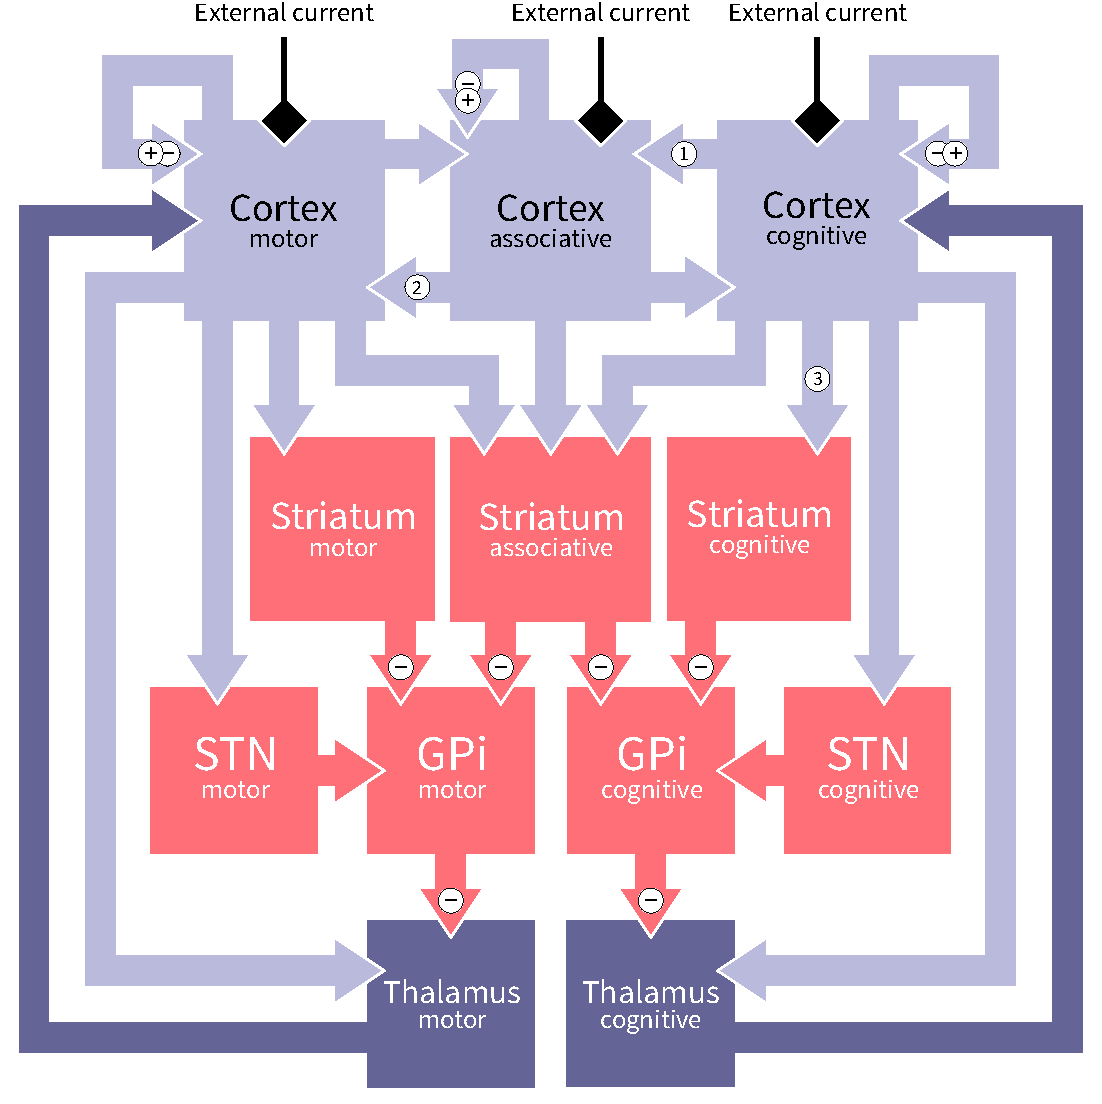
\includegraphics[width=0.5\textwidth]{architecture}
  \caption{Architecture of the model}
  \label{fig:architecture}
\end{figure}



\begin{figure}[h]
        \centering
        \begin{subfigure}[b]{0.3\textwidth}
                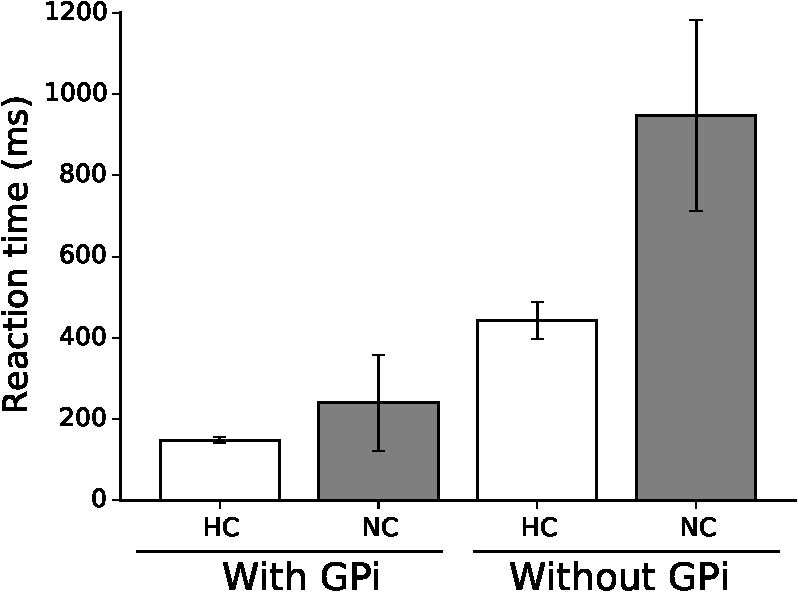
\includegraphics[width=\textwidth]{RTresults}
                \caption{RTresults of the model}
                \label{fig:RTresults}
        \end{subfigure}
        ~ %add desired spacing between images, e. g. ~, \quad, \qquad, \hfill etc.
          %(or a blank line to force the subfigure onto a new line)
          
        \begin{subfigure}[b]{0.5\textwidth}
                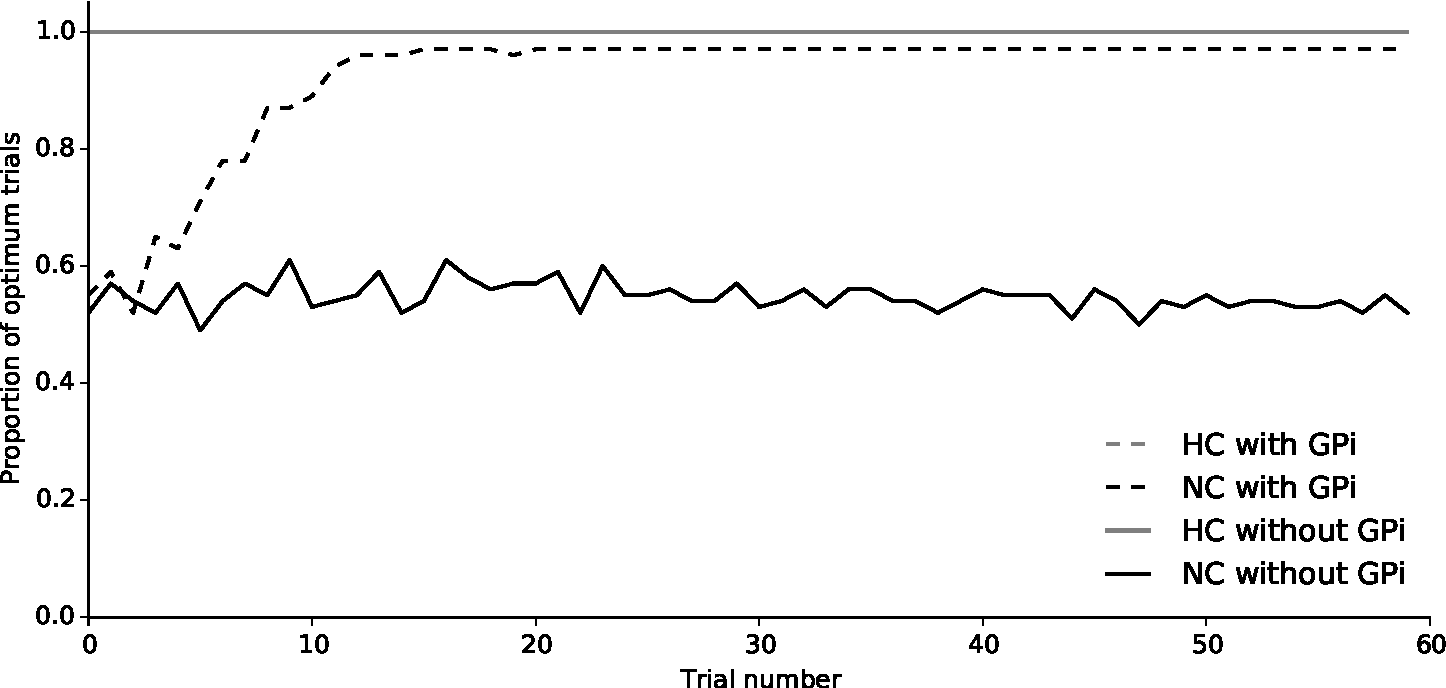
\includegraphics[width=\textwidth]{Performances}
                \caption{Performances of the model}
                \label{fig:Performances}
        \end{subfigure}
        \caption{Results of the model}\label{fig:Results}
\end{figure}



\end{document}
